\section{Résultats expérimentaux}
\subsection{Visualisation des profils de mouvement}
\subsubsection{Profil de mouvement $\frac{1}{2} \frac{1}{2} \frac{1}{2}$}
\begin{figure}[H]
    \centering
    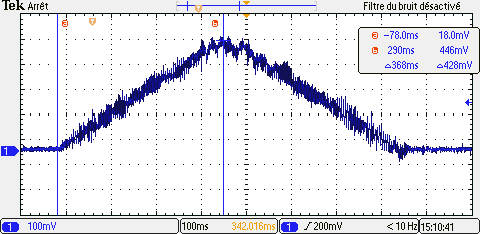
\includegraphics[width=1\linewidth]{Images/PM_triangle_0.75s.PNG}
    \caption{Profil de mouvement $\frac{1}{2} \frac{1}{2} \frac{1}{2}$}
    \label{fig:triangle}
\end{figure}
\subsubsection{Profil de mouvement $\frac{1}{3} \frac{1}{3} \frac{1}{3}$}
\begin{figure}[H]
    \centering
    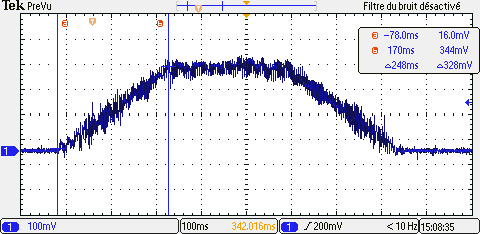
\includegraphics[width=1\linewidth]{Images/PM131313_075s.PNG}
    \caption{Profil de mouvement $\frac{1}{3} \frac{1}{3} \frac{1}{3}$ }
    \label{fig:131313}
\end{figure}
\subsubsection{Profil de mouvement $\frac{1}{6} \frac{2}{3} \frac{1}{6}$}
\begin{figure}[H]
    \centering
    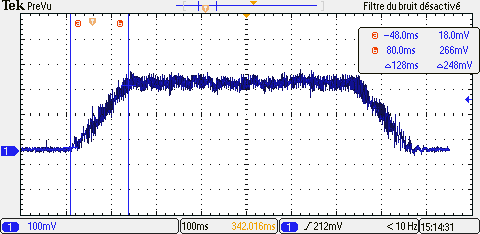
\includegraphics[width=1\linewidth]{Images/PM_162316_075s.PNG}
    \caption{Profil de mouvement $\frac{1}{6} \frac{2}{3} \frac{1}{6}$ }
    \label{fig:162316}
\end{figure}
\subsection{Réduction du temps de mouvement}
\subsection{Bonus : Comparaison de fonctionnement entre micro-pas et pas entiers}
\begin{figure}[H]
    \centering
    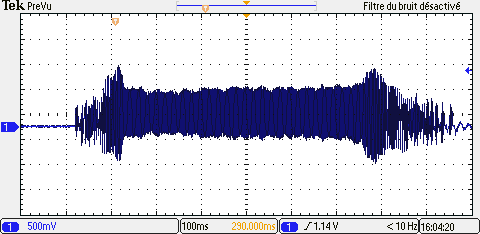
\includegraphics[width=1\linewidth]{Images/bonus_1.PNG}
    \caption{Fonctionnement en pas entiers}
    \label{fig:profil_bonus}
\end{figure}
\begin{figure}
    \centering
    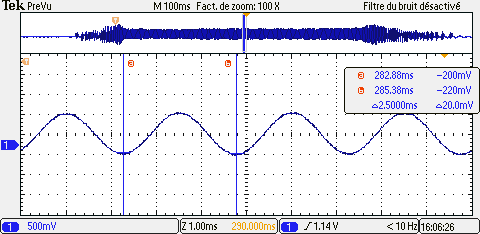
\includegraphics[width=1\linewidth]{Images/bonus_2.PNG}
    \caption{Fréquence d'oscillation en pas entiers}
    \label{fig:freq_bonus}
\end{figure}